In this chapter we review the results obtained through out this work and obtain phyisicaly relevant quantities from our simulations and analytical computations. 

Throughout this work we have explored three different setups. Firstly we explored the case where there is no chemical reaction at the interface. This is the case of normal electrolytes under no external electric field. Secondly we studied the case where current is imposed through the electrolyte solution and therefore reaction is driven by this current. 

Lastly we studied the case where the reaction takes the form of Langmuir isotherm in the limiting case where the constant $K_{eq}S_T << 1$ where $K_{eq}$ and $S_T$ are the equilibrium of the adsorption reaction and the concentration of available sites, respectively. 

An interesting parameter extractable from our models is the relaxation time, or the time it takes the system to reach steady state. Also we are interested in finding how the electric field at the surface varies with bulk concentrations and the electrolytic cell's potential.  We will first analyze steady state solutions and then we will move on to the dynamical system.



\section{Steady State Solution In Forced Current Regime}

Fig. \ref{fig:analytic-results} shows the analytic results while \ref{fig:numeric-results} shows numeric results for the steady state. This results are obtained by numerical evaluation of system \ref{eq:nernst-planck} and perturvatively finding solutions up to first order on a forced current setup as shown in \ref{eq:first-order-system}

\begin{figure}[h!]
 \centering
 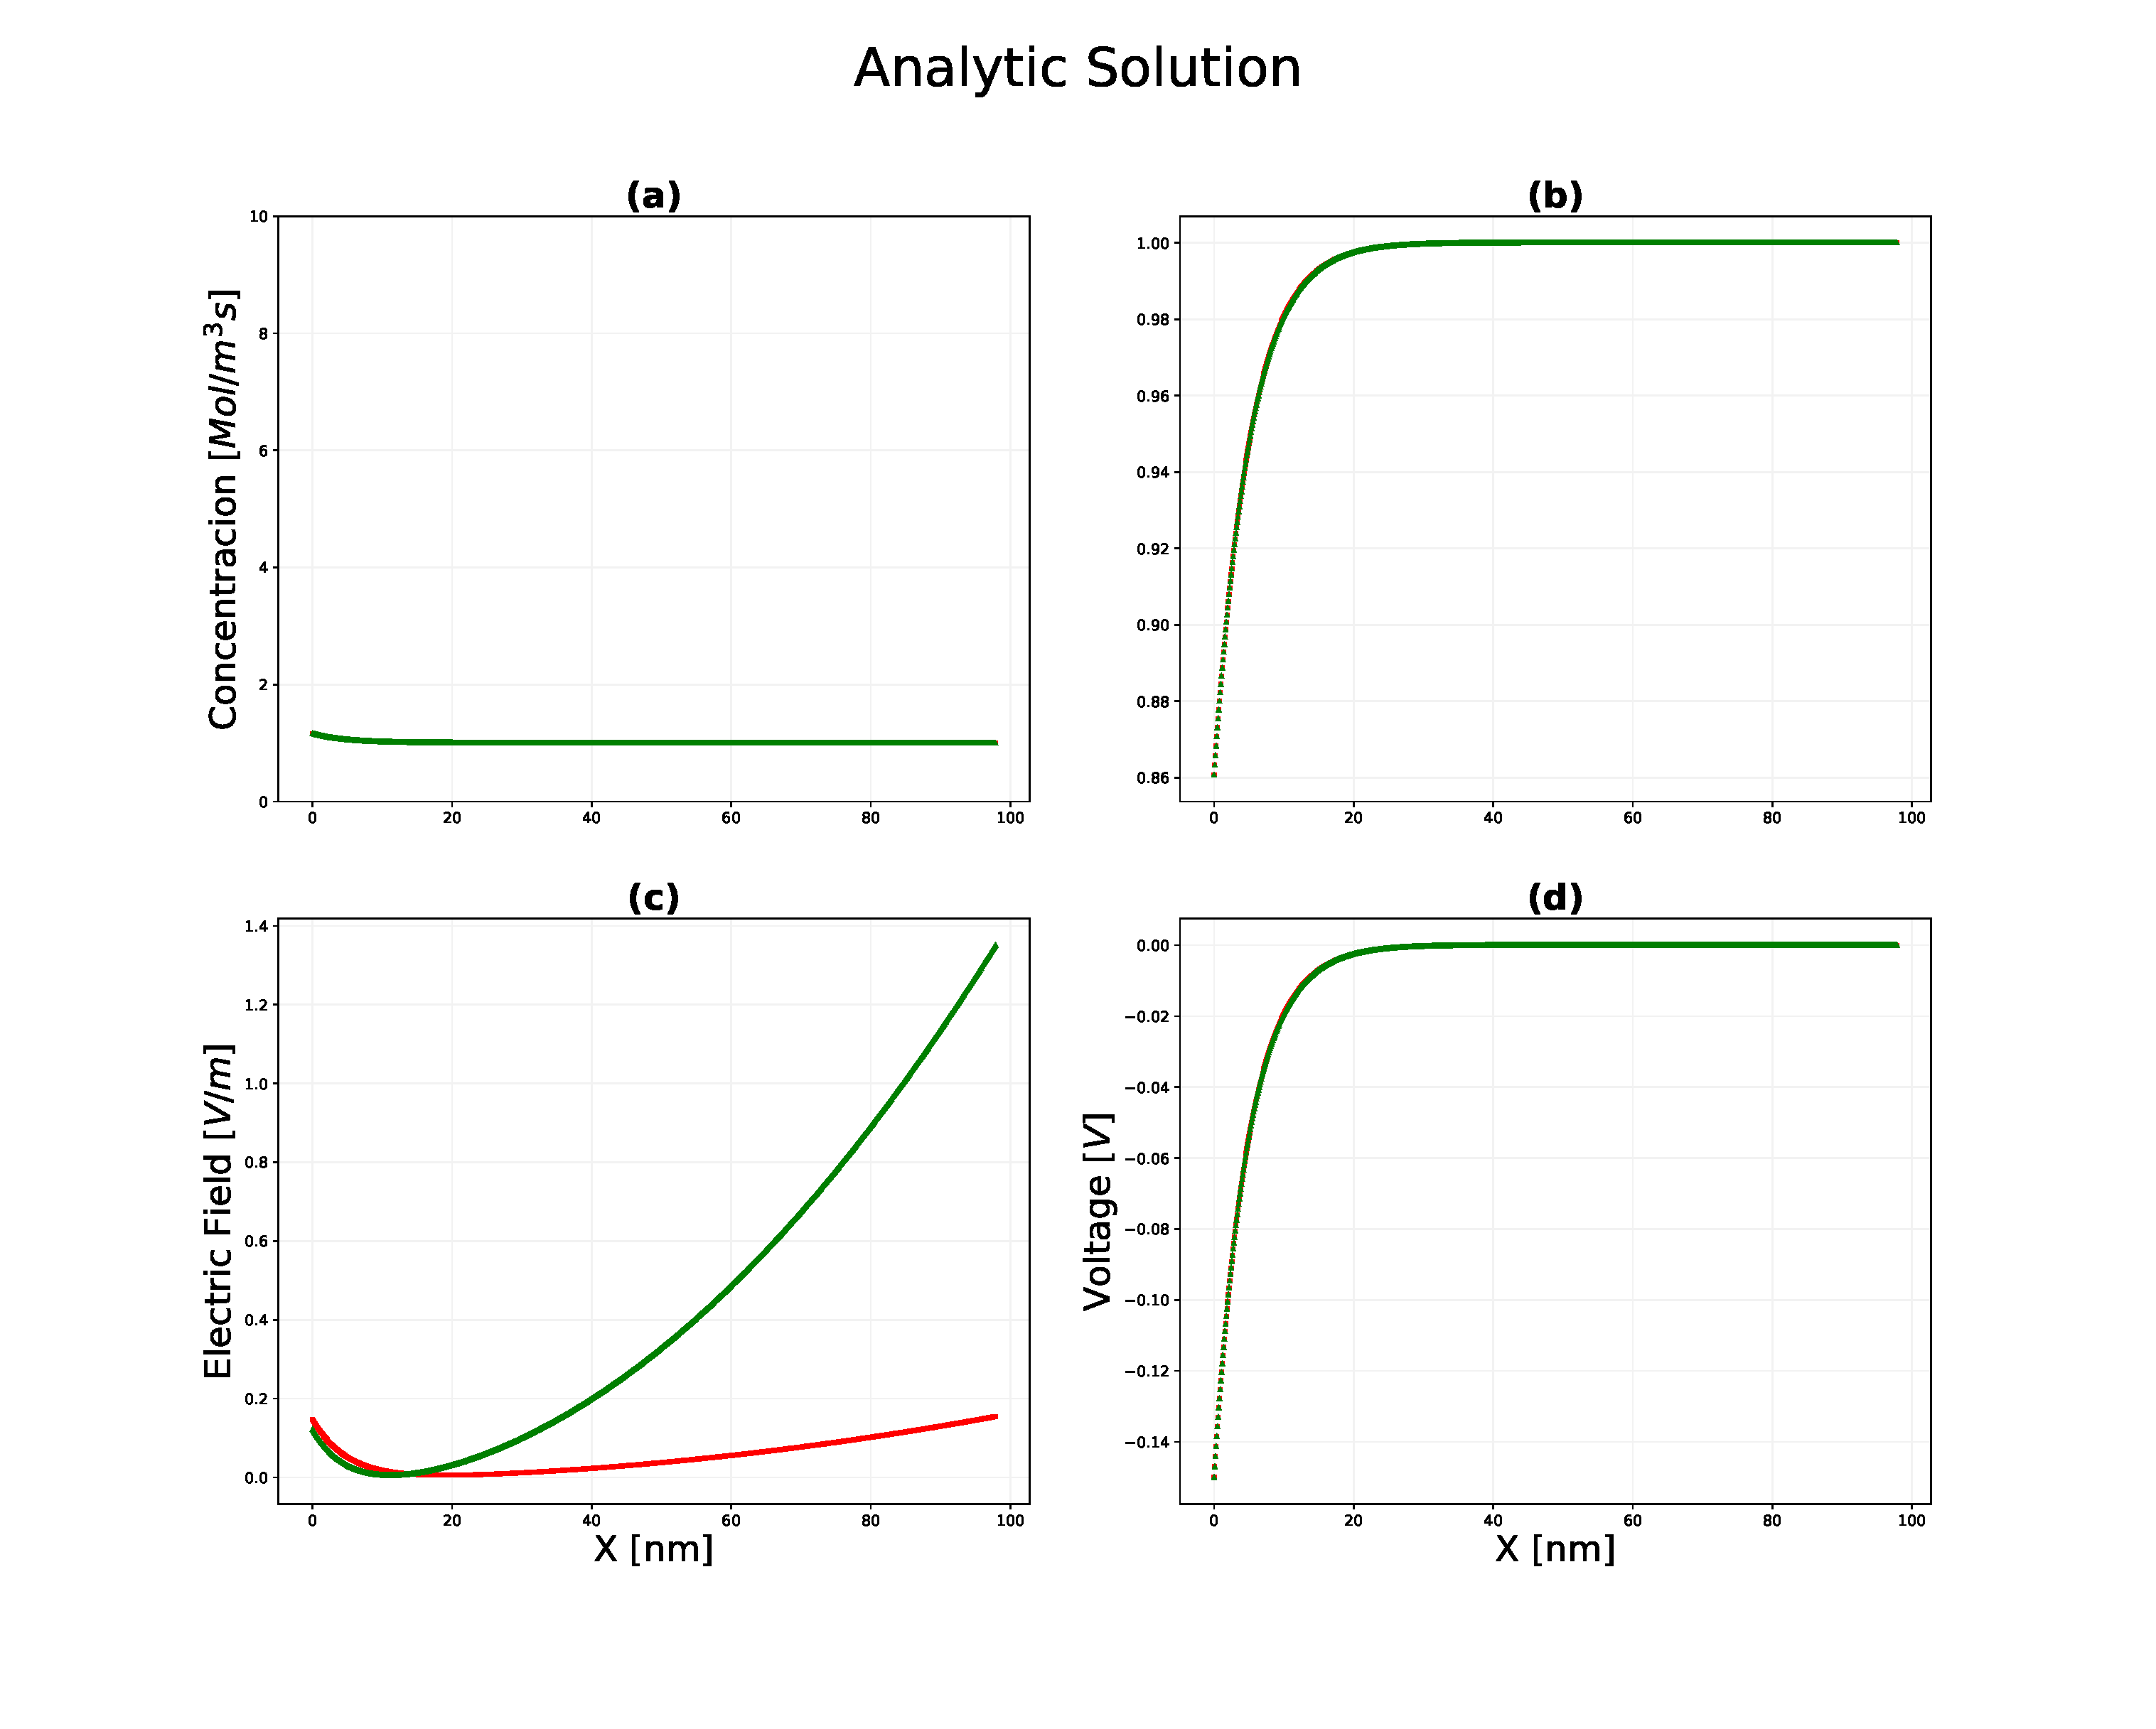
\includegraphics[width = \linewidth]{analytic-results}
 \caption{Analytic results. (a), (b) are the concentrations of each species of electrolytes. (c) is the electric potential and (d) the electric potential. Each plot is compared for 3 different values of the reaction rate. In this case, Cauchy boundary conditions are imposed on the potential and the electric field is computed as proportional to the negative derivative of the electric potential.}
 \label{fig:analytic-results}
\end{figure}


As for the numerical part, Fig. \ref{fig:numeric-results} shows the results obtained. The solution of the steady state at different values of the reaction rate do not defer much closest to the surface of the electrode ($x=0$). Also, from Fig. \ref{fig:numeric-results} (c) and (d) we can see that the aproximation of the electric field and the electric potential is fairly 

\begin{figure}[htbp]
 \centering
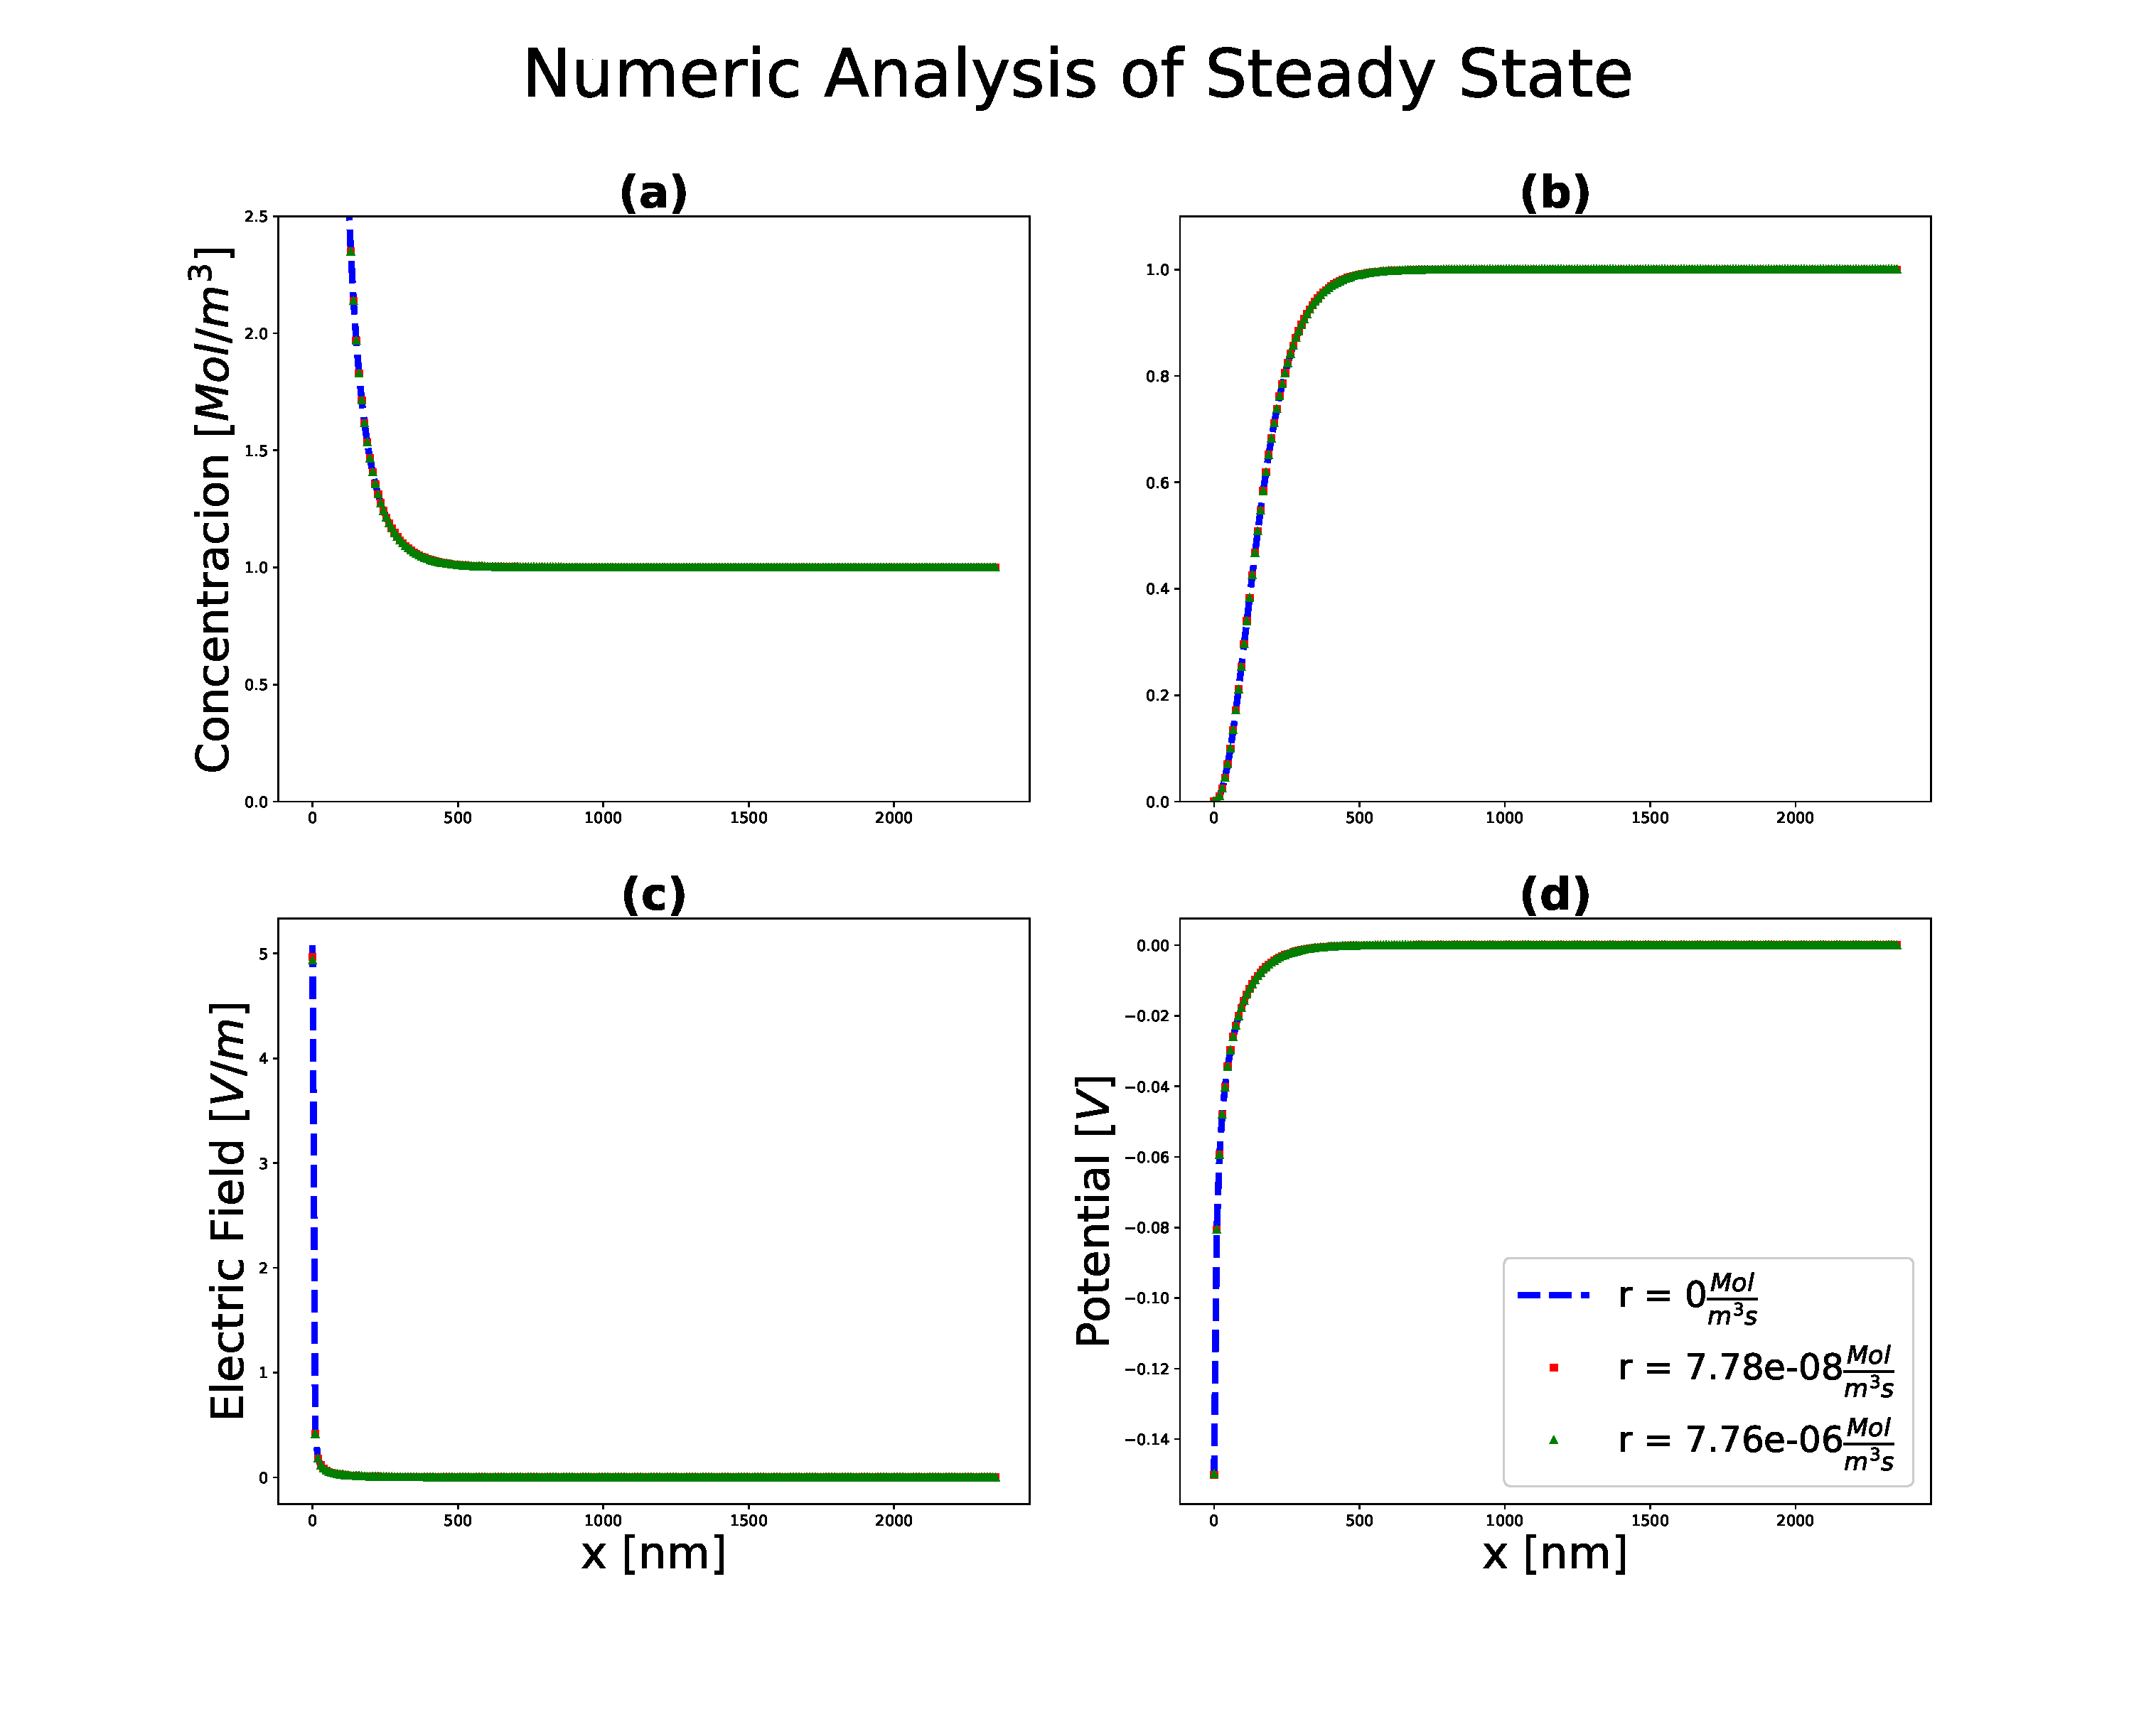
\includegraphics[width = \linewidth]{results-numeric}
 \caption{The numerical solution to the potential to first order in the current. Here, the boundary conditions for the potential are Cauchy boundary conditions in what is known as a two point boundary value problem, but using the Shooting method explained in Section \ref{sec:shooting-method} transform it into a single point boundary value problem. The boundary conditions for the electric field (as it is proportional to the derivative of the potential) are thus computed, not imposed.}
 \label{fig:numeric-results}
\end{figure}

Dealing with the equations as presented in Eq. \ref{eq:system} is extremely difficult when doing a numerical analysis. This is due to the fact that the natural units of the system (x which is measured in meters) are too small for the computer to handle. Also, non-linearity gives extreme fluctuations of the concentration of the positive ion near the surface. Since we where using the shooting method, we needed to change the values of the electric field at the bulk, such that the boundary condition for the electric potential is correct, but this induced such strong concentrations at the interface sometimes, that the computer could not handle the numbers resulting from Runge-Kutta method. We had to make a little adaptation in order to be able to find the correct boundary condition for the electric field with the shooting method. 




As it can be seen in Fig  \ref{fig:numeric-results} $(c)$ and $(d)$, the electric field and potential approach zero when the start moving into the bulk of the solution, as expected. The further away from the interface we go, the better the border conditions for the electric field are met. For our particular case, we cut the integration range when we reached a tolerance of $ E_{bulk} < 1\times 10^{-3}$, where $E_{bulk}$ is the border condition of the dimensionless electric field at the bulk. 



A similar analysis can be done for the concentrations (Fig.  \ref{fig:numeric-results}) $(a)$ and $(b)$), but this time the value of both concentrations at the bulk is $C_b$, as defined by the border conditons for the system \ref{eq:system}.



Another difficulty is that, since we used the adaptive Runge-Kutta method, the concentrations change so abruptly that the adaptive step $h$ becomes increadibly small. The problem with this is that the number of iterations needed with a step of the order of $h\approx 10^{-29}$. In order to reach the full length of integration is too big and therefore, we obtain only a part of the integration interval and not as close to the interface as we should like. 

To avoid such difficulties, we have worked with the adimensional potential in a scale of adimensional length $\xi = \kappa x$. We have integrated on the interval $[0, 20 \kappa \delta]$.




%\begin{figure}[htbp]
%\begin{subfigure}{.5\linewidth}
%\centering
%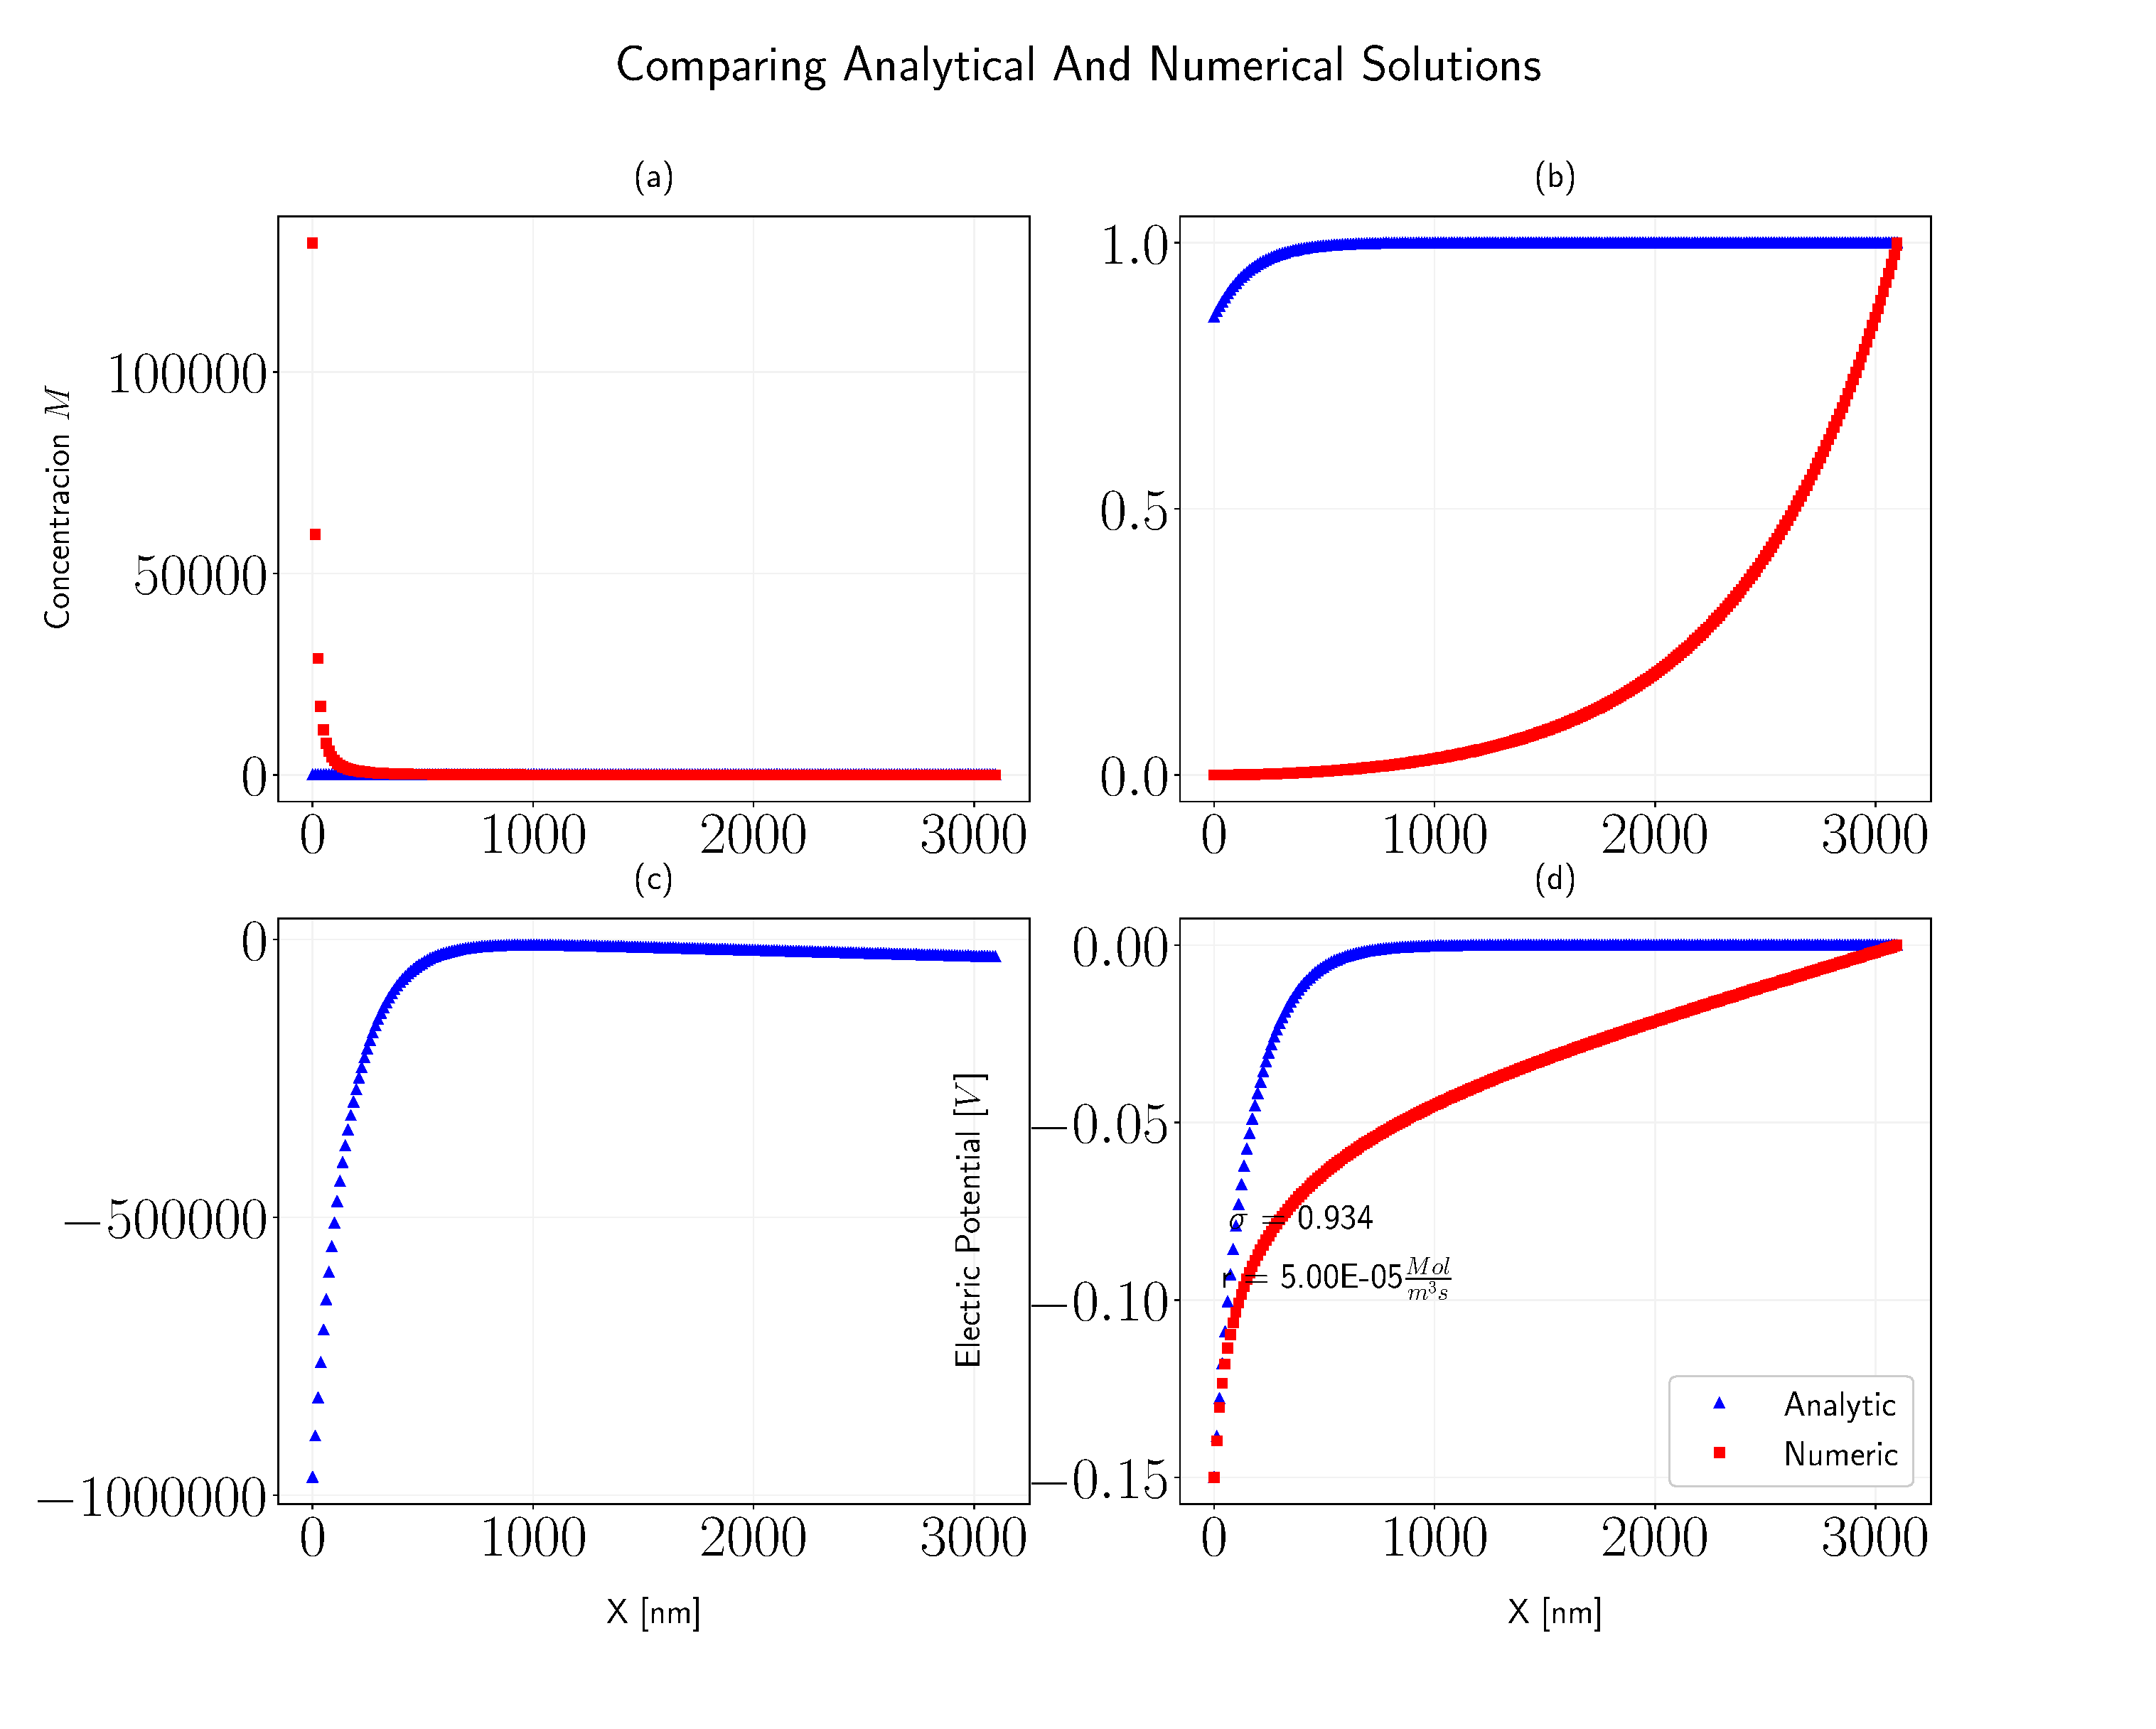
\includegraphics[width=\textwidth]{comparison0}
%\caption{}
%\label{fig:sub1}
%\end{subfigure}%
%\begin{subfigure}{.5\linewidth}
%\centering
%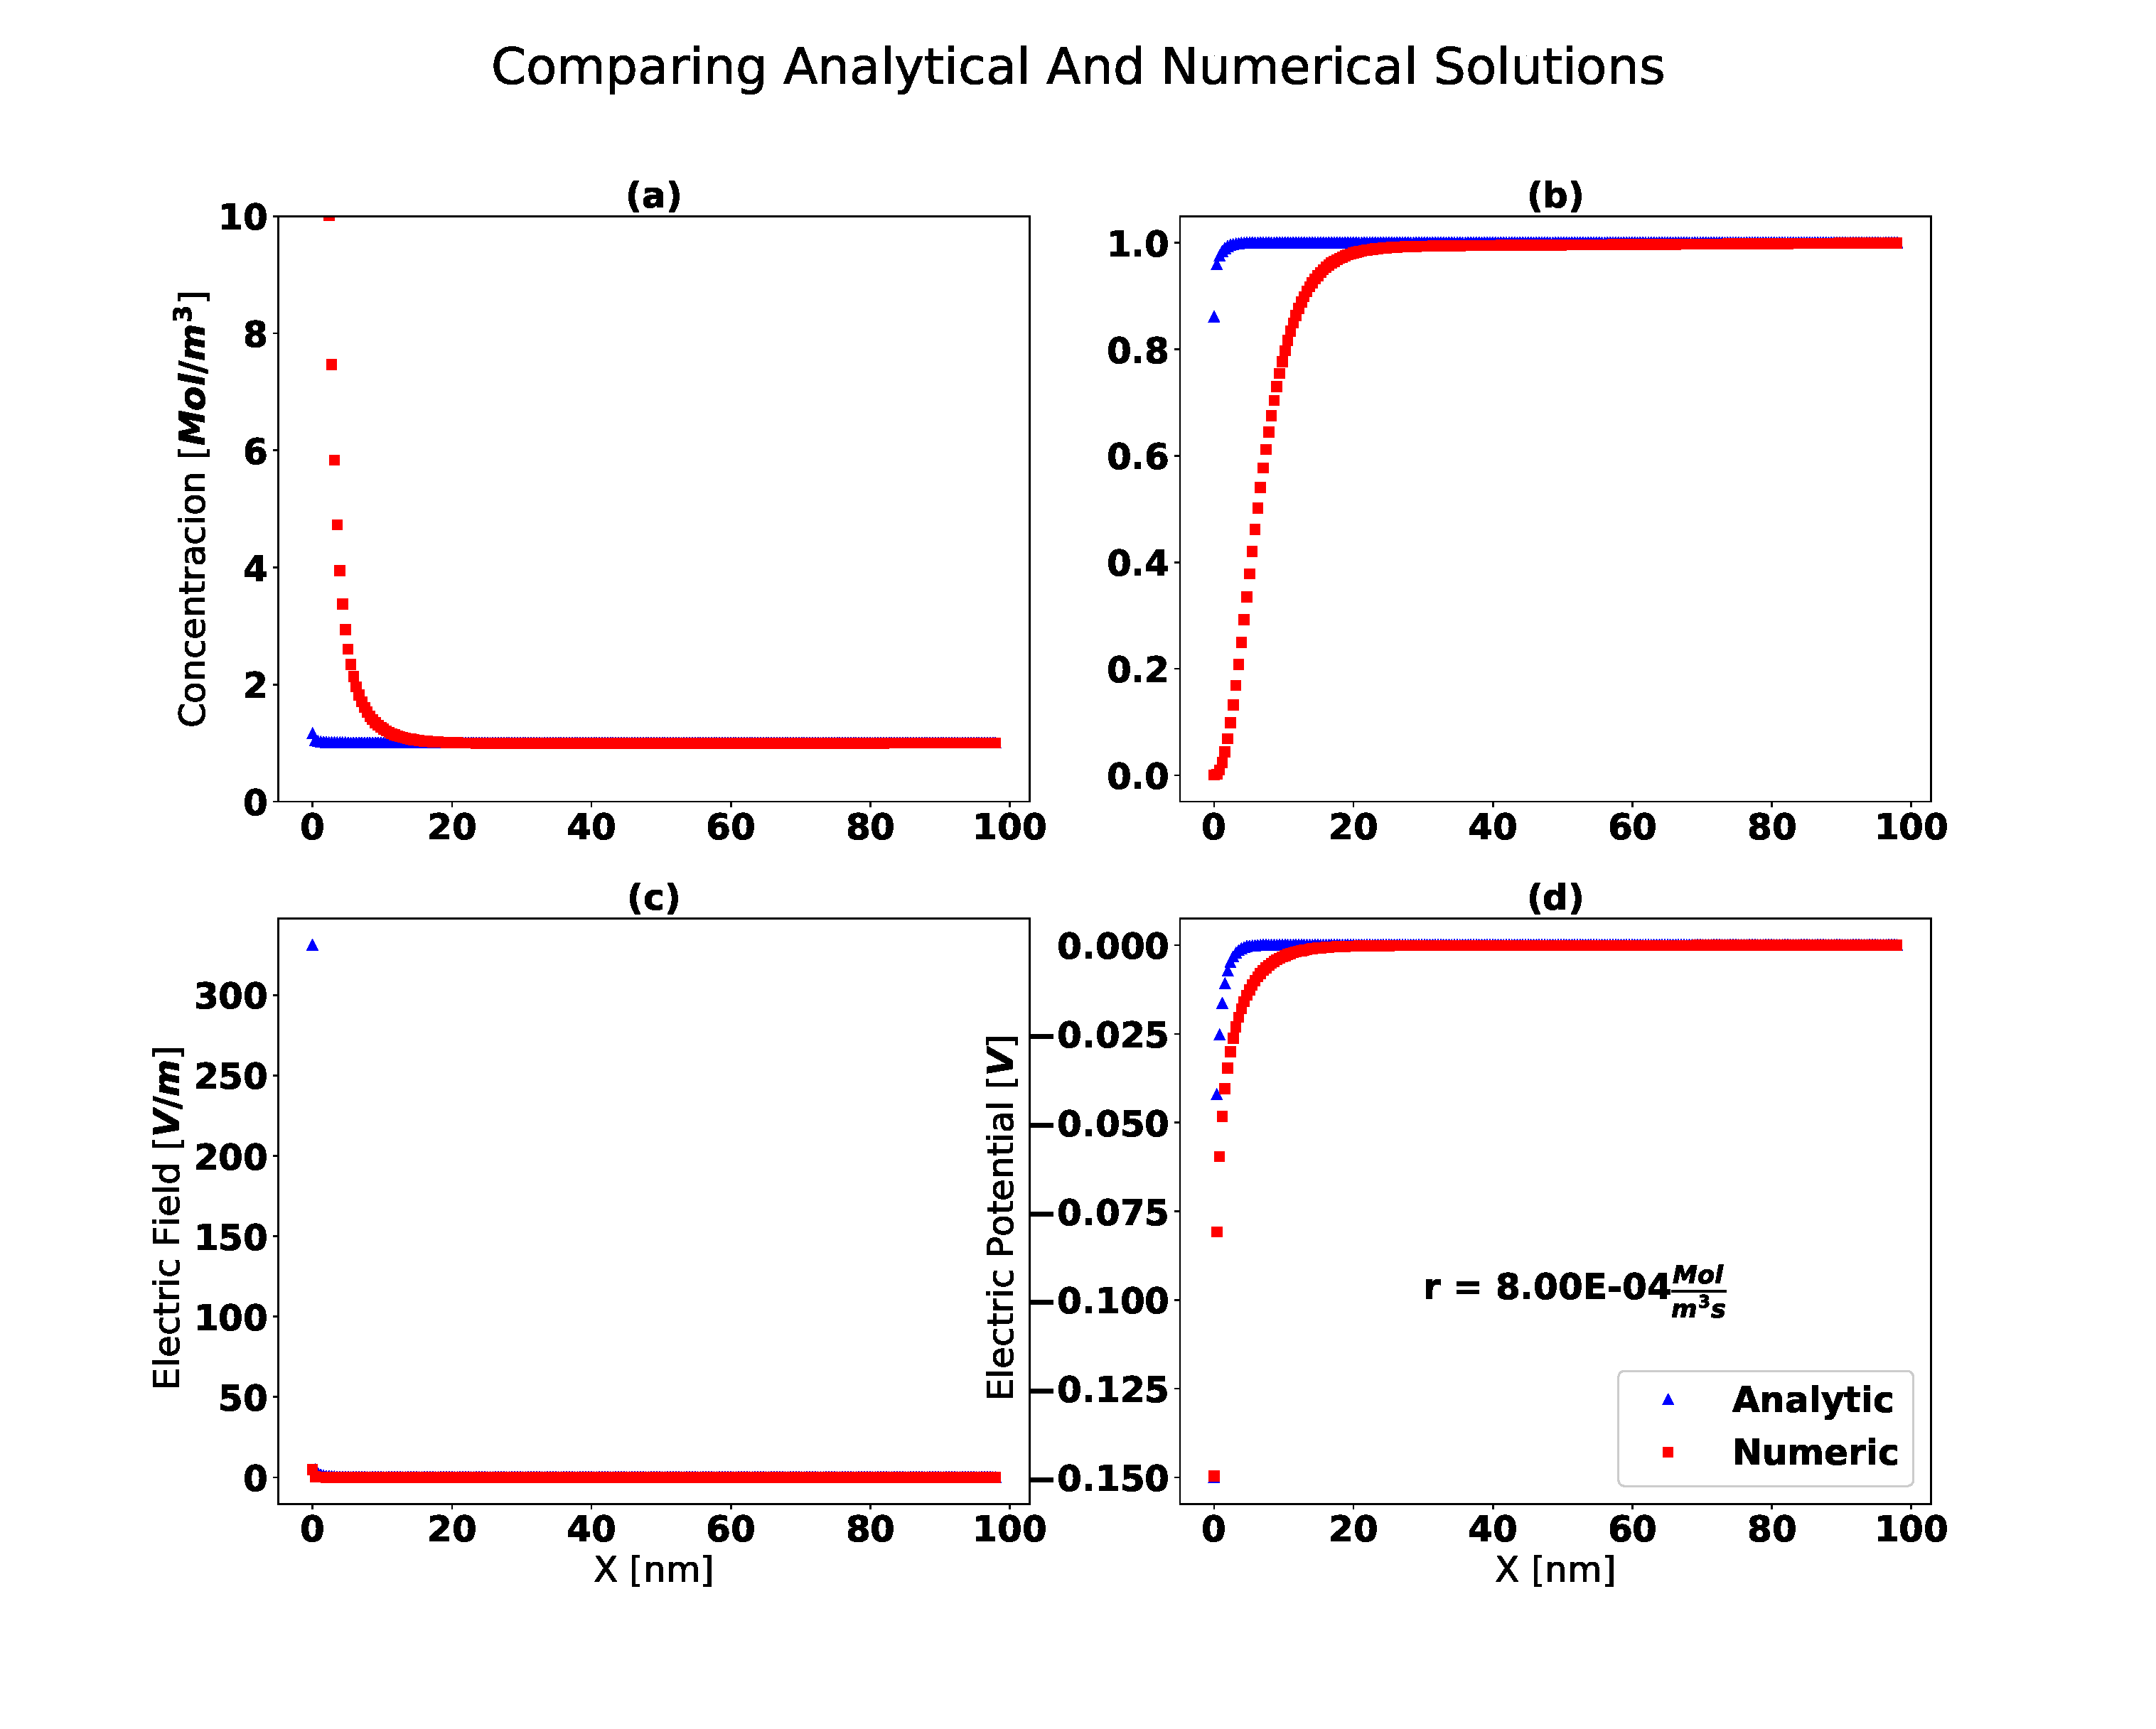
\includegraphics[width =\textwidth]{comparison1}
%\caption{}
%\label{fig:sub2}
%\end{subfigure}\\[1ex]
%\begin{subfigure}{\linewidth}
%\centering
%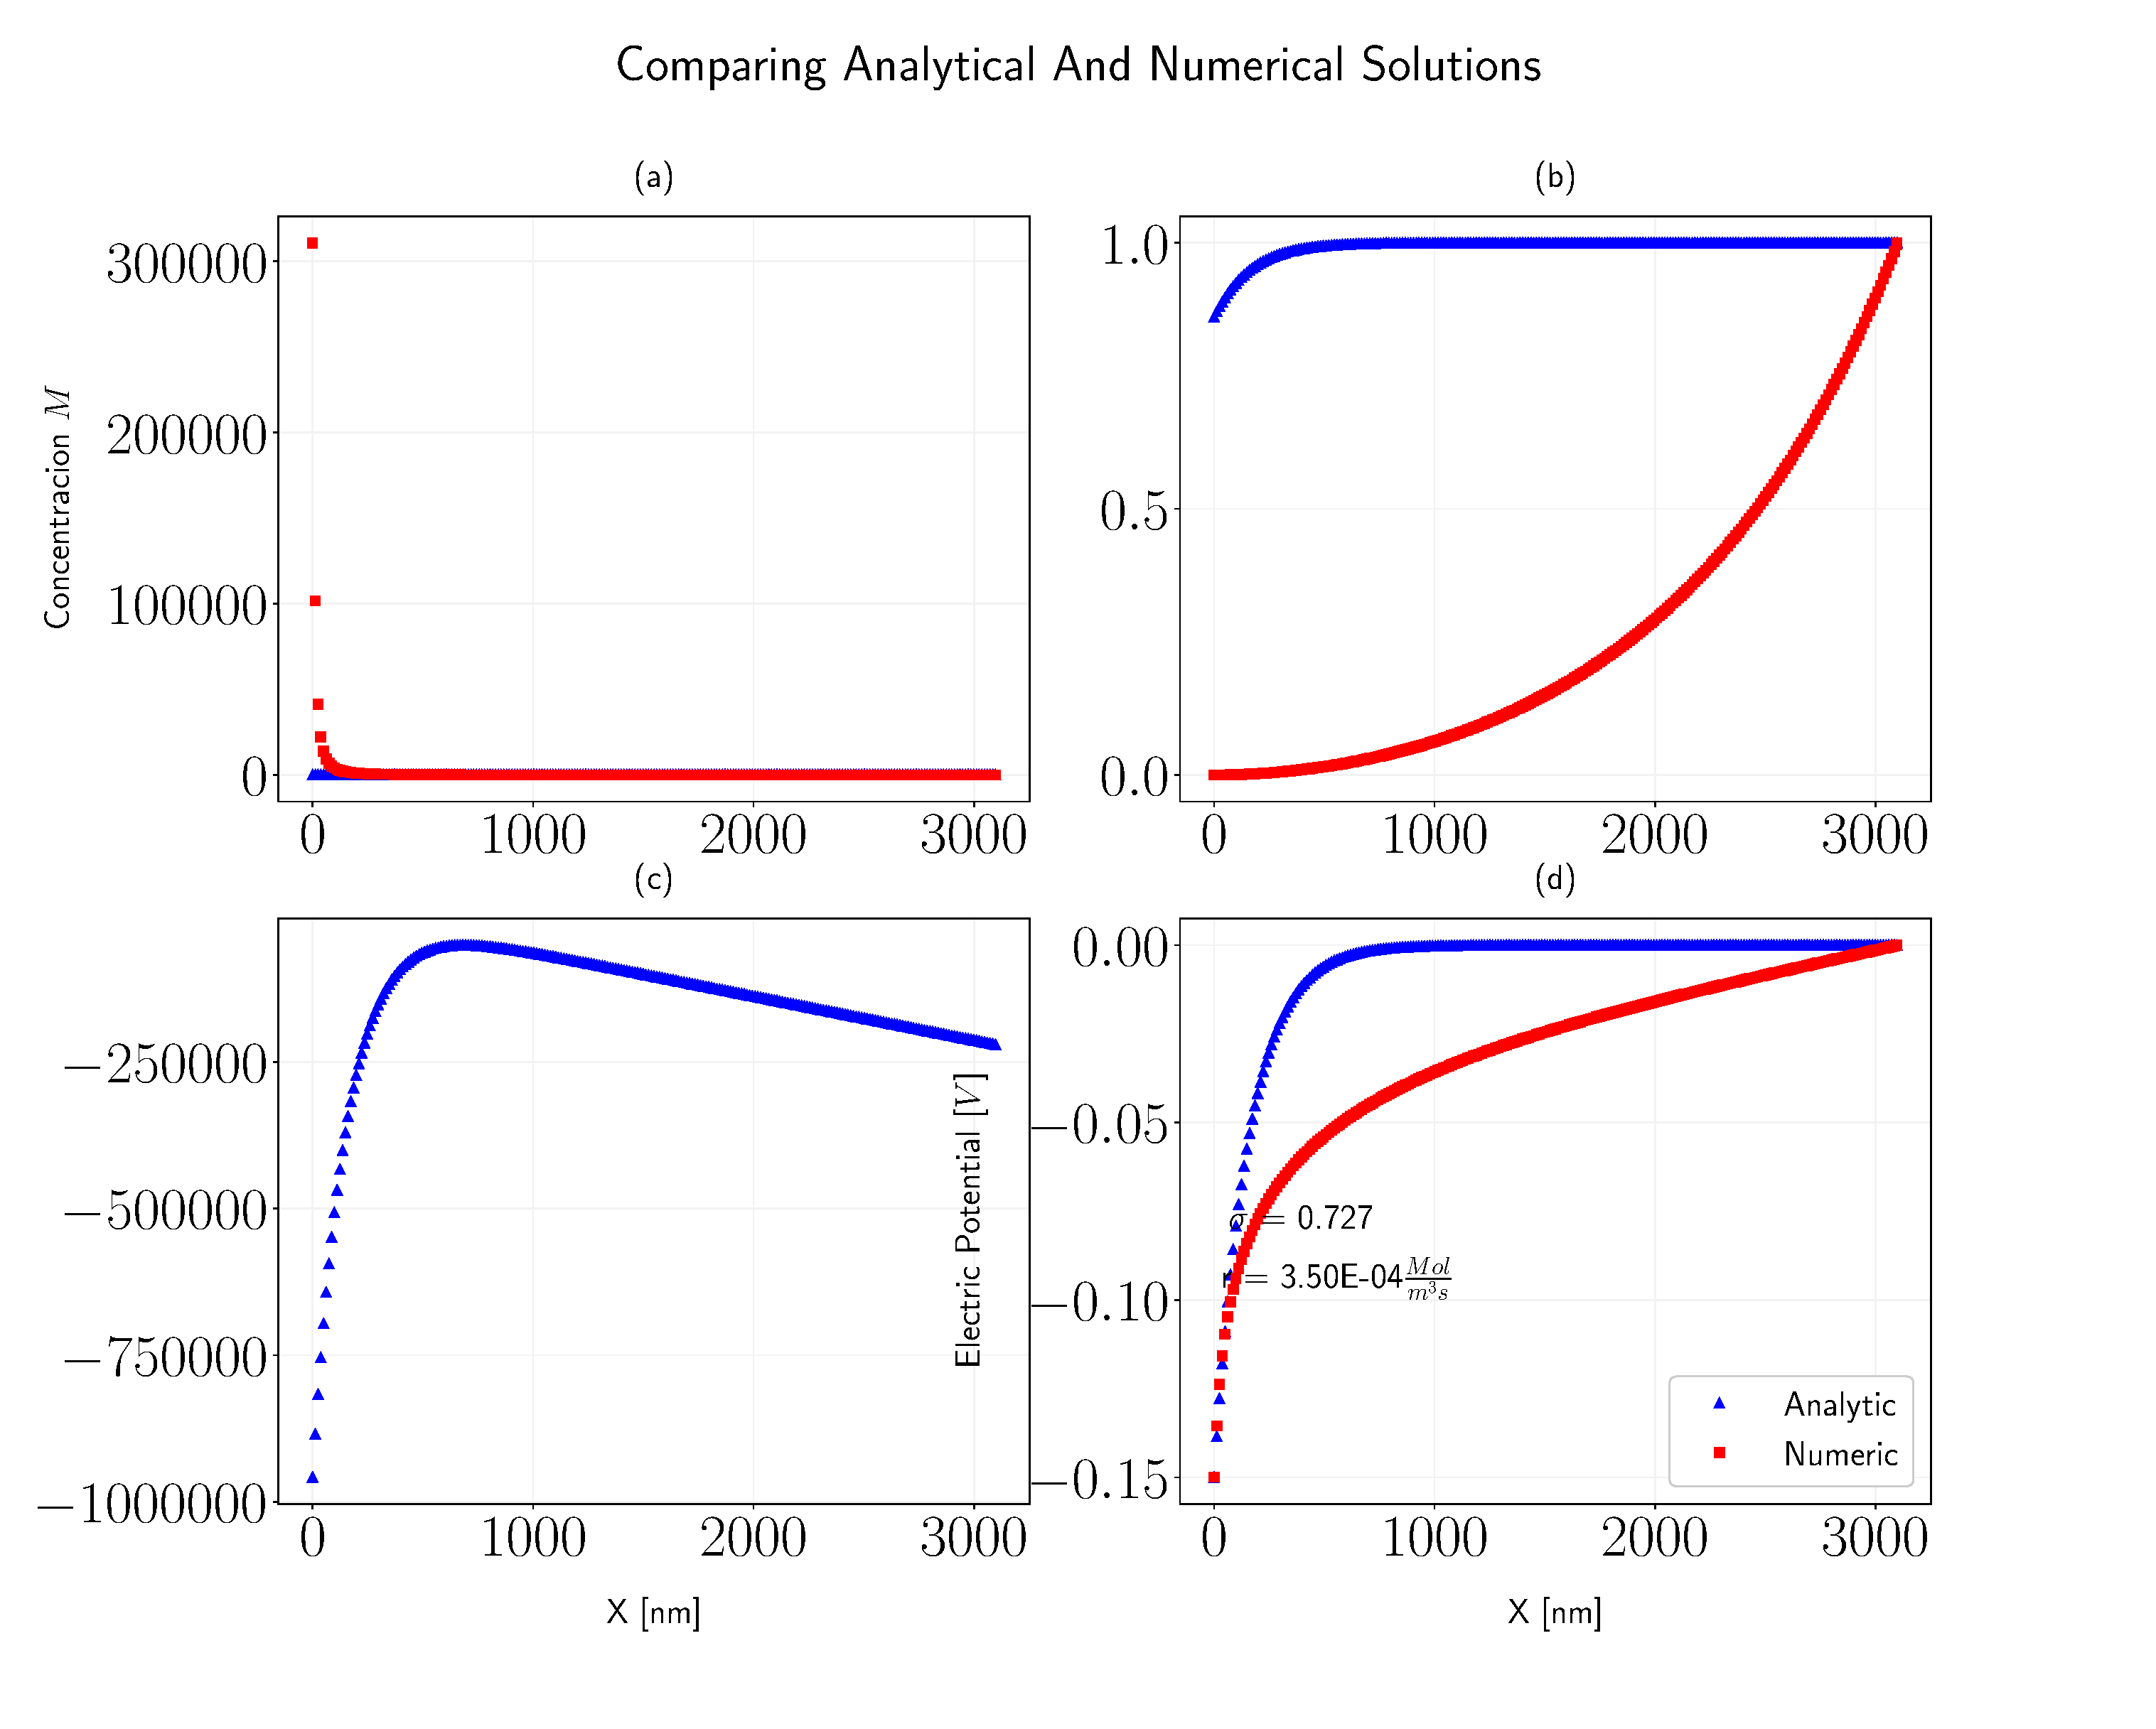
\includegraphics[width =0.5\textwidth]{comparison2}
%\caption{}
%\label{fig:sub3}
%\end{subfigure}
%\caption{Three subfigures}
%\label{fig:comparison}
%\end{figure}


